\documentclass{beamer}
\usetheme{Unistra}
% elimine la barre de navigation tout en haut
\setbeamertemplate{headline}{}
% definit le type de transition d'un transparent au suivant
\addtobeamertemplate{background canvas}{\transdissolve}{}

\usepackage[french]{babel}
\usepackage[T1]{fontenc}

\title{Exemple de presentation}
\subtitle{(avec {\LaTeX} et Beamer)}
\author{Alberto Barsella}
\institute{Universit\'e de Strasbourg}
\date{\today}

\begin{document}

\begin{frame}
\titlepage
\end{frame}

\begin{frame}
\frametitle{Titre de la page}
Lorem ipsum dolor sit amet, consectetur adipisicing elit, sed do eiusmod tempor incididunt ut labore et dolore magna aliqua.

\vspace{1em}
Lorem ipsum dolor sit amet, consectetur adipisicing elit, sed do eiusmod tempor incididunt ut labore et dolore magna aliqua.
\end{frame}

\begin{frame}
\frametitle{Des listes}
\begin{itemize}
    \item le début
    \item $\vec{F} = m\vec{a}$
    \item $W_{A\rightarrow B}(\vec{F}) = \int_{t_{\rm A}}^{t_{\rm B}}\vec{F}\cdot\vec{v}\,\mathrm{d}t$
    \item la fin
\end{itemize}
\end{frame}

\begin{frame}
\frametitle{Des formules}
Selon mon calcul qui est trop bien:
\begin{equation}
    \sum_{i=0}^N \int_0^\infty f_i(x) e^{-x^2}\,\mathrm{d}x = 0 \nonumber
\end{equation}
\end{frame}

\begin{frame}
\frametitle{Des images}
Les chats jouent un rôle important en physique!
\begin{center}
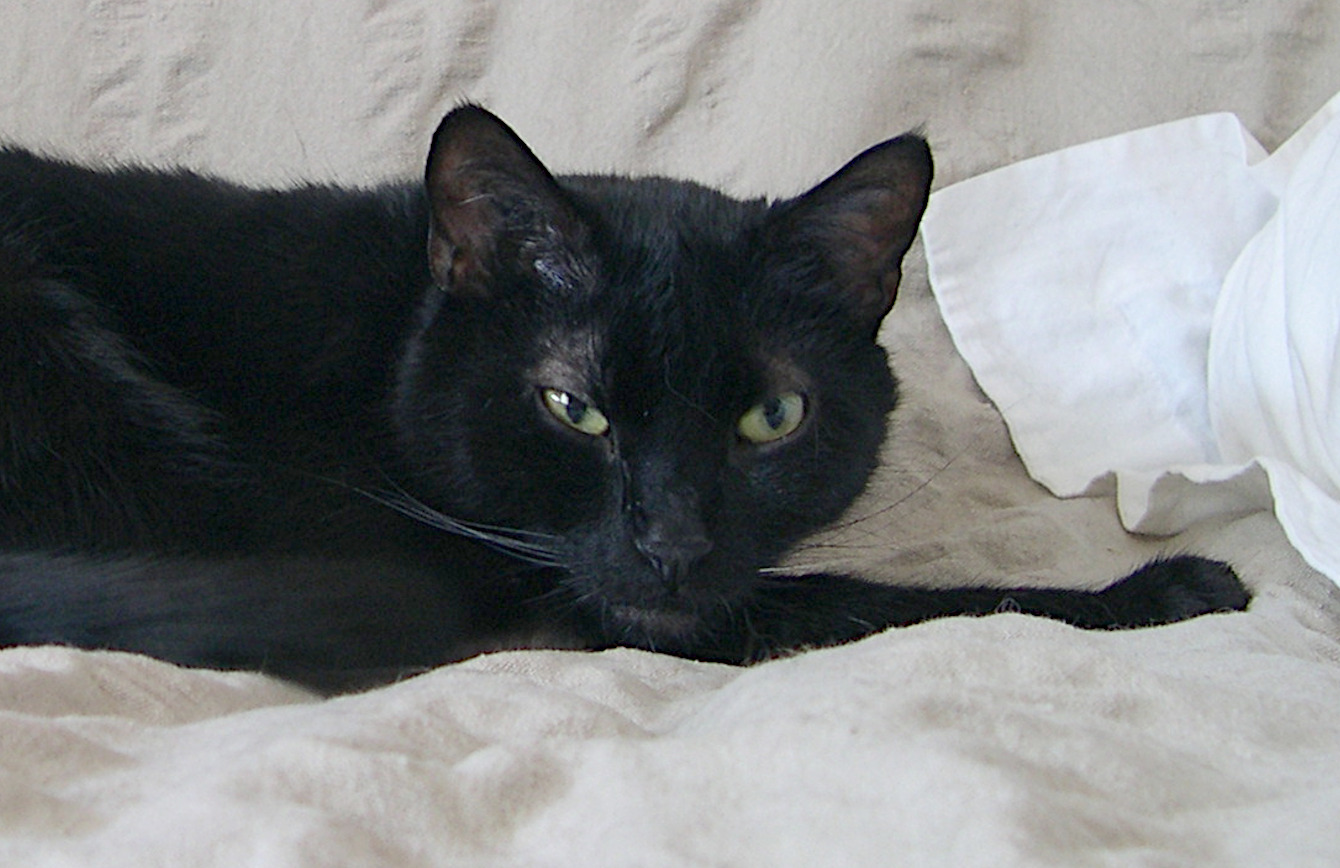
\includegraphics[width=0.6\textwidth]{chat.jpg}
\end{center}
\end{frame}

\begin{frame}
\frametitle{Conclusion}
\begin{enumerate}
    \item Beamer est trop bien
    \pause\item il peut faire apparaître les lignes une à une
    \pause\item ne pas regarder dans le laser avec l'oeil qui vous reste
    \pause\item ne pas essayer d'attraper le chat avec la main qui vous reste
\end{enumerate}
\end{frame}

\end{document}
